\makeatletter
\def\thickhrulefill{\leavevmode \leaders \hrule height 1ex \hfill \kern \z@}
\def\@makechapterhead#1{%
  \vspace*{10\p@}%
  {\parindent \z@ \centering \reset@font
        {\Huge \scshape \thechapter}
        \par\nobreak
        \vspace*{15\p@}%
        \interlinepenalty\@M
        \begin{tabular}{@{\qquad}c@{\qquad}}
          \hline
          \\
          {\Huge \bfseries #1\par\nobreak} \\
          \\
          \hline
        \end{tabular}
    \vskip 100\p@
  }}
\def\@makeschapterhead#1{%
  \vspace*{10\p@}%
  {\parindent \z@ \centering \reset@font
        {\Huge \scshape \vphantom{\thechapter}}
        \par\nobreak
        \vspace*{15\p@}%
        \interlinepenalty\@M
        \begin{tabular}{@{\qquad}c@{\qquad}}
          \hline
          \\
          {\Huge \bfseries #1\par\nobreak} \\
          \\
          \hline
        \end{tabular}
    \vskip 100\p@
  }}

\chapter{Rendszerterv}

\section{Kliens Szerver architektúra} % (fold)
\label{sec:kliens_szerver_architektúra}
\indent A kliens-szerver architektúra üzenet alapú és moduláris felépítésű, ezáltal támogatják a az újrafelhasználhatóságot, rugalmasságot, együttműködési és bővíthetőséget. Jellemzői:
\begin{itemize}
  \item Kéréseket küldünk a szerver felé.
  \item A választ a szervertől kapjuk.
  \item Szerepek: kérő (client) és kiszolgáló (server).
\end{itemize}

\begin{figure}[h!]
  \centering
  % Upper part of the page
	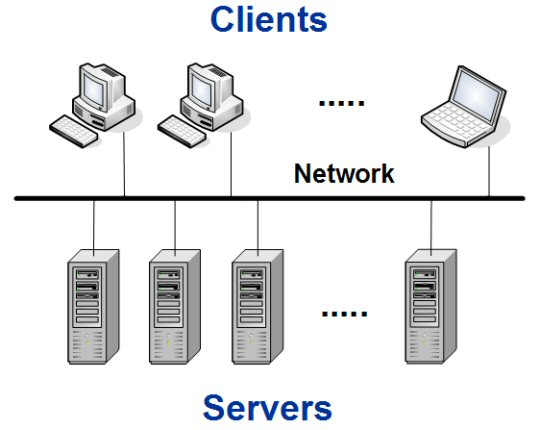
\includegraphics[width=0.5\textwidth]{chapters/chap3/cs.jpg}\\
	\caption{Kliens szerver architektúra}
\end{figure}

  \paragraph{Kliensek} általában alkalmazások vagy eszközök, amelyek szolgáltatásokat kérnek a szervertől, a kapott választ feldolgozva vagy anélkül prezentálják a felhasználó felé, vagy továbbítják a kapott választ egy másik kliens-vagy szerver felé.
Három csoportba sorolhatjuk a klienseket, hogy milyen bonyolultságú és erőforrás igényű egy kliens.
  \begin{description}
    \item[Vékony kliens (Thin client)] minimális eszközökkel rendelkező kliens. A kliensnek szükséges erőforrásokat is a távoli (host) gépen veszi igénybe.
    \item[Vastag kliens (Fat client)] Jellemzője, hogy önmaga hajtson végre nagyobb adatmennyiségekkel feldolgozásokat, amikor a szerver inkább elsődleges tárolóként viselkedik. 2003-as évek elejétől a gazdag kliens (rich client) kifejezést eltérő értelemben kezdték el használni, mint a vastag klienst. Ennél a kliens architektúránál a szerver központi egységének a kihasználtsága sokkal kiegyenlítettebb, mint a többiek esetében. Maga a kliens tulajdonképpen vastag kliens, de jobban kihasználja a hálózati lehetőségeket a vékony klienshez hasonlóan, így tulajdonképpen egy vastag-vékony kliens hibrid. Lásd gazdag Internet alkalmazás és gazdag kliens platform.
    \item[Hibrid kliens (Hybrid client)] Hasonlít a vastag klienshez, mivel lokálisan dolgozik, de számít a szerverre adattárolás miatt. Ez a megközelítés sajátosságokat kínál mind a vastag kliensből (multimédia támogatás, nagy teljesítmény), mind a vékony kliensből(erőteljes menedzselhetőség, rugalmasság).
  \end{description}

  \paragraph{Kiszolgáló - Szerver} % (fold)
  Kliens-szerver architektúrában, szerver program kéréseket szolgál ki. Háttér számításokat végez, amelyeket a kliens kért, a választ vissza küldi a kérőnek. Kliensek futhatnak ugyanazon a gépen ahol a szerver, vagy hálozaton keresztül kommunikál a szerverrel.
  \begin{figure}[h!]
    \centering
    % Upper part of the page
  	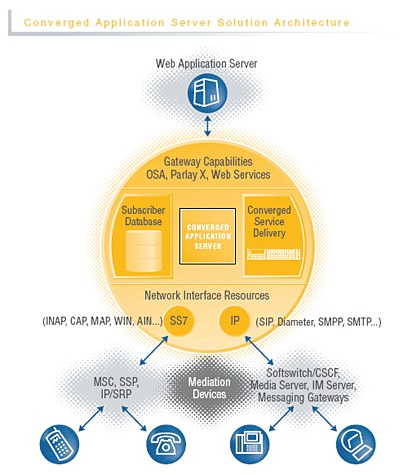
\includegraphics[width=0.4\textwidth]{chapters/chap3/appserver.jpg}\\
  	\caption{Kliens szerver architektúra}
  \end{figure}

% section kliens_szerver_architektúra (end)

\section{Adattárolás} % (fold)
\label{sec:adattárolás}
  Jelenleg három választási lehetőségünk van a nyílt forráskódú adatbázisrendszerek közül, amelyek elterjedtek, jól dokumentált, megbízható és nem utolsósorban rendelkeznek térbeli függvények támogatásával:
  \begin{enumerate}
    \item MySQL
    \item Spatialite
    \item PostgreSQL
  \end{enumerate}
	\subsection{MySQL} % (fold)
	\label{sub:mysql}
	Egy nagyon fontos kritérium, a helyes működéshez MyISAM szerkezetűnek kell lennie minden táblának. MyISAM támogatást ad egyaránt spatial és nem spatial adatokra.
	
	Spatial Extension funkciók:
	\begin{itemize}
		\item Geometria model támogatás: polygon, multipoint, linestring, curve, \ldots
		\item Adatok formátumok WKT (Well known text), WKB (Well known binary)
		\item Geometria függvények.
	\end{itemize}
	Úgy éreztem használati szempontjából egy kicsit körülményes volt.
	% subsection mysql (end)

	\subsection{Spatialite} % (fold)
	\label{sub:spatialite}
	Gyors, egyszerű, kicsi, hordozható. Egy hátránya van, nem képes konkurensen működni. Úgy gondolom fontos megemlíteni, mert
	nagyon hatékonyan lehet adatokat tárolni, rengeteg nyelven írtak API-t SQLite adatbázishoz. Spatialite extension-je pedig szinte minden
	geometria függvényt lefed, amit MySQL adatbázis motor szolgáltat.
	% subsection spatialite (end)
	
	\subsection{PostgreSQL - Postgis} % (fold)
	\label{sub:postgresql}
	Postgres adatázishoz külön telepíthető komponens. Hatékony, nyíltforráskódú adatbázisrendszer.
	
	Spatial extension funkciók:
	\begin{itemize}
		\item Geometria model támogatás: teljes.
		\item Adat formátumok: WKT, WBT.
		\item Geometria függvények.
		\item Adatkezelő felület: ERSI, SVG adatok import és export funkciók.
		\item Bulk Loader: tömeges adatok feltöltése.
		\item Third party szoftver támogatás: QGis, Grass, \ldots
	\end{itemize}
	Három adatbázis motor közül PostreSQL-re esett a választásom.
	% subsection postgresql (end)
	
	A következő címeken linkeken lehet elérni a fent említett adatbázisrendszereket:
	\begin{center}
	    \begin{tabular}{ | l | l | p{5cm} |}
		\hline
	    \hline
	    Adatbázisrendszer Neve & Leírás \\ \hline
	    MySQL & \url{http://www.mysql.com/} \\ \hline
 		Spatialite & \url{http://www.gaia-gis.it/spatialite/} \\ \hline
 		PostgreSQL & \url{http://www.postgresql.org/} \\ \hline
	    Postgis & \url{http://postgis.refractions.net/} \\ \hline
	    \hline
	    \end{tabular}
	\end{center}

  Elsőre a MySQL megfelelőnek tűnik, azonban az igényeket felmérve, a következő feltételeket nem tudja teljesíteni:
  \begin{itemize}
    \item Spatial kiegészítője még nagyon kezdetleges funkcionalítással rendelkezik.
    \item Nem tudja lefedni a spatial műveletek többségét.
    \item Nagy adathalmaz esetén már lassúvá válik.
  \end{itemize}
  Mivel a PostgreSQL adatbázisrendszerhez PostGIS kiegészítés tartozik, amely a térbeli adattípusok , különböző vetületi rendszerek , térbeli műveletek , adatformátumok közti konverzió szolgáltatásokkal rendelkezik, így PostgreSQL adatbázisrendszerre esett a választás.
  
  
  Ezenkívül a PostgreSQL nagyon jól dokumentált és rengeteg példa kóddal rendelkezik.
  Több programozási nyelvhez van Application Programming Interface (API).
  
% section adattárolás (end)

\section{Kliens oldali vektoros megjelenítő és szerkesztő} % (fold)
\label{sec:gis_kiegészítő}
Az alkalmazáshoz  olyan megjelenítő eszközt kell találni, amelynek használatához kevés gyakorlatot igényel vagy előképzettség szükségeltetik.
Erre jelenleg:
\begin{enumerate}
  \item Google Maps API \footnote{https://developers.google.com/maps/}
  \item Yahoo Maps API \footnote{http://developer.yahoo.com/maps/}
  \item Bing Maps API \footnote{http://www.microsoft.com/maps/developers/web.aspx}
  \item OpenLayers \footnote{http://openlayers.org/}
\end{enumerate}
Kiválasztásuknál a következő szempontokat kellett vizsgálni:
\begin{itemize}
  \item API támogatás.
  \item Jól dokumentált.
  \item Ingyenesen elérhető.
  \item Geometriai objektumok szerkeszthetősége.
  \item Adatformátumok támogatása import és export esetekben.
\end{itemize}
Ezek közül az OpenLayers bizonyult a legjobbnak, így ráesett a választás. A következő lépések szükségesek a térkép megjelenítéséhez.
\begin{enumerate}
  \item OpenLayers inicializálás.
  \item Térkép réteg megadás, amely lehet WMS (Web Map Service) vagy szolgáltatók által megadott API-n keresztül.
  \item Vektoros réteg inicializálás.
  \item Szerkesztési kontrollok inicializálása és callback függvények implementálása.
  \item Adatformátumok definiálása.
\end{enumerate}
Mivel ezt a műveletet mindig végre kell hajatni, ha egy térképet szeretnék használni, kód megismétlődés, újrafelhasználhatóság szempontokból is ajánlott volt kitenni egy külön osztályba, amely a térképi funkciókért felelős. Ez így is történt, létrejött az \emph{OpenLayersMap} osztály.
\begin{verbatim}
  /**
   * @name OpenLayersMap
   * @param String Div container.
   * @param Array Layers identifier (at least one layer required).
   * @param Array Controls names (optional).
   * @return OpenLayersMap.
   * @author Nguyen Thai Binh.
   */
OpenLayersMap(String container, Array layers, Array Controls) 
    returns OpenLayersMap

    addCamMap = new OpenLayersMap(
        'map', 
        ['osm', 'seccam', 'vect'], 
        ['drag', 'vect', 'polygon', 'modify']);
    init = new initializeListeners(addCamMap);
\end{verbatim}
% section gis_kiegészítő (end)

\section{Webes keretrendszer} % (fold)
A keretrendszer kiválasztásakor a következő szempontok kerültek előtérbe:
\begin{itemize}
	\item Web alapú: Webes keretrendszer.
	\item Moduláris: Egy egyszerű keretrendszer, amelyhez később igény szerint más komponensek csatlakoztathatóak.
	\item Rugalmas: Bővíthetőség valamit külső nem keretrendszerbeli komponensekkel való együttműködés.
	\item Grafikus elemek kezelése.
\end{itemize}
Ezen szempontokat figyelembe véve a következő keretrendszereket vizsgáltam meg:
\begin{enumerate}
	\item Akelos
	\item JEE
	\item Flash CS4
	\item Ruby on Rails
\end{enumerate}

	\subsection{Akelos} % (fold)
	\label{sub:akelos}
	% content section
	
	MVC (Model, Controller, View) keretrendszer PHP-ban. 
	\\
	Magas szintű API-k. Ruby On Rails alapján lett klónozva, feleslegesnek éreztem, hogy
	egy másik szkript nyelvet tanuljak meg, ahhoz, hogy ugyanazt elérjem Ruby On Rails-ben, amit már ismerek, így nem esett rá a választás. 
	% subsection symphony (end)

	\subsection{JEE} % (fold)
	Java Enterprise termékek vizsgálati céljából JBoss rendszer válaszottam, mivel kiforrott, és megbízható.\\
	\label{sub:jee}
			

	Nagyon igéretesnek tűnt, főleg Hibernate rugalmassága és Java nyelv miatt. A következő komponenseit néztem meg:
	\begin{enumerate}
		\item Hibernate: rugalmas adat generálási és elérési réteg.
		\item Open Faces: felhasználói komponensek könyvtára.
		\item JBoss Application Server: alkalmazás szerver.
		\item Google Maps plugin: kiegészítő modul google maps-hez.
	\end{enumerate}
	Azonban a Faces engine kiszámíthatatlan viselkedése javascript-ekkel, le kellett mondanom. Mivel Google Maps API-ja javascriptben íródott
	, használata javascript megbízható működését igényel.
	% subsection  (end)
	
	\subsection{Flash CS4} % (fold)
	\label{sub:flash_cs4}
	
	Grafikai szempontokat teljesen jól teljesítette, azonban egy nagyon nagy problémája van. Az adatok elérése adatbázison
	keresztül nagyon körülményes, számomra használhatatlan. Adatbázis kezelés php file-okon keresztül lehet megvalósítani POST/GET
	metódusokon keresztül.
	% subsection flash_cs4 (end)

\label{sec:webes_keretrendszer}

\subsection{Ruby on Rails} % (fold)
\label{sub:ruby_on_rails}
Ruby on Rails webes keretrendszert választottam. A Ruby on Rails (röviden Rails) a Ruby programozási nyelvre épülő, nyílt forrású (MIT licenc alatti) webalkalmazás-keretrendszer. David Heinemeier Hansson írta 2004-ben, a Basecamp program kódjának felhasználásával.

\paragraph{Technikai háttér}
Alapelvei a Don't repeat yourself (ne ismételd magad) és a Convention over Configuration (konvenciók a beállítások előtt): minden információ csak egy helyen szerepel (például egy adatbáziskezelő osztályban nem kell az oszlopokat definiálni, a Rails közvetlenül kiolvassa a nevüket az adatbázisból), és a konvenciókat követő elnevezésekhez automatikusan kódot generál a rendszer (például az adatbázis sales táblája automatikusan hozzárendelődik a Sale osztályhoz). AJAX-támogatása miatt a web 2.0 alkalmazások egyik népszerű keretrendszere.

\paragraph{Az alkalmazás futtatása}
Noha a WEBrick, a Rubyban írt webszerver nagyon jó tesztelésre, kész alkalmazások futtatására, különösen nagy terhelés alatt nem alkalmas. A kész alkalmazások deploymentjéhez több megoldás kínálkozik. A Mongrel mellett lehetőség van lighttpd-n vagy IIS-en futtatni az alkalmazásokat. Ugyanakkor a Mongrel parserére, a Rack és az Event Machine-re épített Thin sebessége miatt kedvelt választás. Azonban a deployment könnyedsége miatt a Phusion Passenger lett a hivatalosan ajánlott platform. Ezzel Apache vagy Nginx szerveren futtathatjuk a Rails keretrendszerben írt alkalmazásunkat.

\paragraph{Keretrendszer struktúrája}
A Ruby on Rails keretrendszer különböző csomagokat tartalmaz, mint az
\begin{description}
  \item[ActiveRecord] Objektum relációs leképezésért felelős csomag.
  \item[ActionController] Kérések feldolgozása és válasz küldés kliensnek.
  \item[Html ERB] Megjelenítés és Elrendezésért felelős csomag.
  \item[ActionMailer] Email szolgáltatásokért felelős csomag.
\end{description}
Ezeken kívül bárki készíthet kiegészítéseket az alapcsomagok kibővítésére. Ahhoz, hogy a térbeli adatokat könnyen tudjam használni valamint térbeli kereséseket tudjak végezni, felhasználtam a következő kiegészítő csomagokat:
\begin{enumerate}
  \item \emph{gem 'pg'} PostgreSQL adatbázis driver.
  \item \emph{gem 'rgeo'} Geometriai objektumok kezeléséért felelős csomag \footnote{https://github.com/dazuma/rgeo}.
  \item \emph{gem 'rgeo-geojson'} Geometriai objektumok geojson adatformátumba való konvertálásáért felelős csomag.
  \item \emph{gem 'rgeo-activerecord'} Geometriai objektumok relálciós leképezéséért felelős.
  \item \emph{gem 'activerecord-postgis-adapter'} PostGIS kiegészítőhöz  objektum relációs leképező driver.
\end{enumerate}

  Felhasználók kezelését pedig \emph{gem 'devise'} \footnote{https://github.com/plataformatec/devise } csomagot használtam fel.
  
  \paragraph{Az MVC architektúra}
	\emph{Model}: Active Record osztály a model réteg magja. Ezen keresztül szinte bármilyen adatbázissal tudunk dolgozni. 
	Alkalmazás írása közben is meg van a lehetőség, hogy adatbázis motort változtassunk mivel a kapcsolatot egy yml fileban van tárolva
	és Migration modul segítségével bármikor vissza tudjuk állítani a sémát egy másik adatbázison.
	
	
	\emph{View}: Active View osztály felel a megjelenítésért. html.erb kiterjesztés megadja a lehetőséget, hogy egyszerre natív html, javascript
	valamint ruby kódot tudjunk futtatni. 
	
	
	\emph{Controller} Moduláris komponensekre lehet osztani az alkalmazást. Minden egyes kontroller saját funkcionalitásáért felelős, igy struktúráltabb
	és átláthatóbb a kód.
	% subsection ruby_on_rails (end)
	
	A következő címeken linkeken lehet elérni a fent említett keretrendszereket:
	\begin{center}
	    \begin{tabular}{ | l | l | p{5cm} |}
		\hline
	    \hline
	    Keretrendszer Neve & Leírás \\ \hline
	    Akelos & \url{http://www.akelos.org/} \\ \hline
 		JEE & \href{http://www.oracle.com/technetwork/java/javaee/tech/index.html}{Oracle JEE} \\ \hline
	    Flash CS4 & \url{http://www.adobe.com/products/flash/} \\ \hline
	    Ruby on Rails & \url{http://rubyonrails.org/} \\ \hline
	    \hline
	    \end{tabular}
	\end{center}

% subsection ruby_on_rails (end)

\section{Projekt struktúra} % (fold)
\label{sec:projekt_struktúra}
Egy rails projekt három fontos könyvtárból áll:
\begin{itemize}
	\item \emph{app}
	\item \emph{db}
	\item \emph{public}
\end{itemize}

  \subsection{db könyvtár} % (fold)
  \label{sub:db_könyvtár}
  Ebben vannak az adatbázissal kapcsolatos definíciós file-ok találhatóak, nevezetesen:
  \begin{enumerate}
  	\item \emph{schema.rb}: Séma leíró file.
  	\item \emph{migrate}: ebben a könyvtárban található az adatbázis séma változtatásának verziói. Lehetőséget ad arra, hogy tetszőleges 
  	séma verzióra álljunk vissza.
  \end{enumerate}
  Szintén adatbázissal kapcsolatos definíciós file a \emph{config/database.yml}, amely adatbázis kapcsolatot definiál mind három fejlesztési fázisra:
  \begin{enumerate}
  	\item Development
  	\item Test
  	\item Production
  \end{enumerate}
  \lstinputlisting[language=SQL]{chapters/chap3/database.yml}

  \begin{figure}[h!]
    \centering
    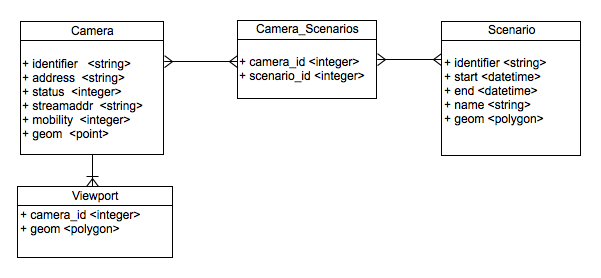
\includegraphics[width=1.0\textwidth]{chapters/chap3/db.png}
    \caption{Adatbázis terv - Entity diagram}
  \end{figure}

  
  Három fő táblára és két kapcsoló van szükségünk:
  \begin{enumerate}
    \item Camera: Kamerák helyzetének és leíró adatainak tárolására.
    \item Viewport: Egy adott kamerához tartozó látómezőinek geometriai adatai.
    \item Scenario: Egy eseményhez tartozó leíró adatok.    
  \end{enumerate}
  

  
  % subsection db_könyvtár (end)


	\subsection{app könyvtár} % (fold)
	\label{sub:app_könyvtár}
	Controller, View, Helper, Model osztályok kódja található. A controller adja a logikai megvalósítást. A modelben található az
	adatbázis objektumokra vonatkozó leképezési objektumok. A helperben olyan osztályok találhatóak, amelyek a megjelenítésben adnak segítséget,
	itt olyan objektumokra, vagy kód szegmensekre gondolok, amelyeket gyakran használunk. A viewben találhatjuk meg az rhtml file-okat.
	
	\paragraph{Camera ActiveRecord}
	Camera objektum reláció leképező model. A szokványos SQL lekérdezéseket implementálja alapértelmezésben, valamint kiegészítve:
	\begin{enumerate}
	 \item wkt: Geometria objektum Well-known-text adatformátum lekérés.
	 \item geom\_collection: Geometria objektum és hozzátartozó összes viewport geometria objektum lekérése WKT formátumban.
	\end{enumerate}
	
	\paragraph{Scenario ActiveRecord}
  Scenario objektum reláció leképező model. A szokványos SQL lekérdezéseket implementálja alapértelmezésben, valamint kiegészítve a \emph{wkt} geometria objektum WKT formátum lekérése.
	
	\paragraph{Camera Controller}
	Kamerával kapcsolatos kérések feldolgozása mint egy adott kamera objektum WKT (Well-known-text-format) formátum lekérése az adatbázisból.
	Funkciói:
	\begin{enumerate}
	 \item Kamera létrehozása.
	 \item Kamerák lekérése.
	 \item Kamerák keresése.
	 \item Kamera módosítása.
	 \item \emph{ajax} Kamerák aszinkron dinamikus lekérése.
	\end{enumerate}
	
	\paragraph{Scenario Controller}
	Eseménnyel kapcsolatos kérések feldolgozása és kiszolgálása.
	Funkciói:
	\begin{enumerate}
	 \item Esemény létrehozása.
	 \item Esemény módosítása.
	 \item Események keresése: dátum szerint, név szerint, azonosító szerint.
	 \item Adott területen levő összes kamerák lekérése.
	 \item Adott eseményben résztvevő kamerák sorrendjének beállítása és elmentése.
	\end{enumerate}
	
	\paragraph{Application Helper}
  Megjelenítést segéd függvényeket tartalmazó osztály.
  Funkciói:
  \begin{enumerate}
    \item Dátumok parse-olása.
	  \item Kamerák állapotától függően a megfelelő ikon hozzárendelése.
	  \item Kamerák mobilitásától függően a megfelelő ikon hozzárendelése.
  \end{enumerate}
	
	\subsection{public könyvtár}
	\label{sub:public_könyvtár}
	Publikus tartalom, mint javascript, grafikai file-ok, html file-ok.
	Itt található olyan segéd könyvtárak mint:
	\begin{enumerate}
	 \item OpenLayers - térkép megjelenítése és szerkesztésért felelős javascript könyvtár.
	 \item JQuery - javascript könyvtár.
	 \item JQuery UI - user interface-el kapcsolatos javascript könyvtár.
	 \item Icons - ikonok könyvtára.
	\end{enumerate}
	
	\paragraph{JQuery} % (fold)
	JQuery egy gyors, robusztus, könnyen használható javascript könyvtár. DOM fa szerkezetet könnyedén lehet kezelni elem id-re vagy class id-re hivatkozva.
	Például:
	\begin{verbatim}
		        $("#element_id")
		        $(".class_id")
	\end{verbatim}
	A DOM elem lekérése után, már meghívhatjuk a natív html függvényeket vagy külső javascript library-ket a kiválasztott elemre.
	% subsection jquery (end)

	% subsection public_könyvtár (end)

% section projekt_struktúra (end)

% section segéd_komponensek (end)

  
% section webes_keretrendszer (end)

\section{Térkép szerver} % (fold)
\label{sec:térkép_szerver}
\paragraph{GeoServer} egy nyíltforráskódú szerver, Java nyelven íródott. Digitális térképek szolgáltatására alkalmas 
WMS (Web Map Service) \footnote{http://en.wikipedia.org/wiki/Web\_Map\_Service} és WFS (Web Feature Service) \footnote{http://en.wikipedia.org/wiki/Web\_Feature\_Service} szolgáltatásokat keresztül.

\paragraph{Célja} Térinformatikai adatok szolgáltatása Webes felületen keresztül.

\paragraph{Tulajdonságai}
Különböző adatformátumokat támogat mint:
\begin{enumerate}
  \item PostGIS
  \item Oracle Spatial
  \item ArcSDE
  \item DB2
  \item MySQL Spatial
  \item ESRI Shape file.
  \item GeoTIFF
\end{enumerate}
Exportálási adatformátumai  lehetnek: KML, GML, ESRI Shapefile, GeoRSS, PDF, GeoJSON, JPEG, GIF, SVG, PNG és még sok más multiméediás tartalom.
% section térkép_szerver (end)

  
